\documentclass[aspectratio=169,12pt]{beamer}
\mode<presentation> {
  \usetheme{metropolis}
}

\usepackage{lipsum}
% \usepackage[colorgrid,gridunit=pt,texcoord]{eso-pic}
\usepackage[absolute,overlay]{textpos}
\usepackage{pythonhighlight}
\usepackage[absolute,overlay]{textpos}
\usepackage{url}
\usepackage{caption}
\usepackage{hyperref}
\usepackage[
    type={CC},
    modifier={by},
    version={3.0},
]{doclicense}

\lstset{
language = Python,
breaklines = true,
basicstyle=\fontsize{7}{7}\selectfont\ttfamily,
commentstyle = {\itshape \color[cmyk]{1,0.4,1,0}},
keywordstyle = {\bfseries \color[cmyk]{0,1,0,0}},
stringstyle = {\ttfamily \color[rgb]{1,0,0}},
frame = single,
}
\hypersetup{
colorlinks=true,
}

\title{Visualize 3D scientific data in a Pythonic way like matplotlib}

\begin{document}
\author{Tetsuo Koyama}
\institute{PyVista developer team}
\date{Python Charity Talks in Japan 2021.09}

\frame{\titlepage}
\note{Hi my name is Tetsuo Koyama. Today I will talk about the title "Visualize 3D scientific data in a Pythonic way like matplotlib".}

\begin{frame}[fragile]
\begin{textblock*}{350pt}(50pt, 20pt)
\begin{block}{Who am I?}
\note{Let me introduce myself first.}
\end{block}
\end{textblock*}
\begin{textblock*}{350pt}(50pt, 70pt)

\includegraphics[width=0.25\linewidth]{tkoyama010.png}
\end{textblock*}
\begin{textblock*}{350pt}(50pt, 170pt)

\includegraphics[width=0.05\linewidth]{twitter-5662063_1280.png}
\end{textblock*}
\begin{textblock*}{350pt}(70pt, 175pt)
\href{https://twitter.com/tkoyama010}{@tkoyama010}
\end{textblock*}
\begin{textblock*}{350pt}(50pt, 200pt)

\includegraphics[width=0.05\linewidth]{github.png}
\end{textblock*}
\begin{textblock*}{350pt}(70pt, 205pt)
\href{https://github.com/tkoyama010}{@tkoyama010}
\end{textblock*}
\begin{textblock*}{350pt}(150pt, 25pt)
\begin{itemize}
\item Mechanical simulation software engineer.
\note{I am mechanical simulation software engineer in my careers.}
\item Stuff of Scipy Japan 2020.
\note{And I was a stuff of Scipy Japan 2020 in community.}
\item PyVista developer team member.
\note{Also I am a member of PyVista developer team.}
\item Science Python Anime and Manga.
\note{I love Science Python Anime and Manga.}
\end{itemize}
\end{textblock*}
\begin{textblock*}{350pt}(200pt, 120pt)
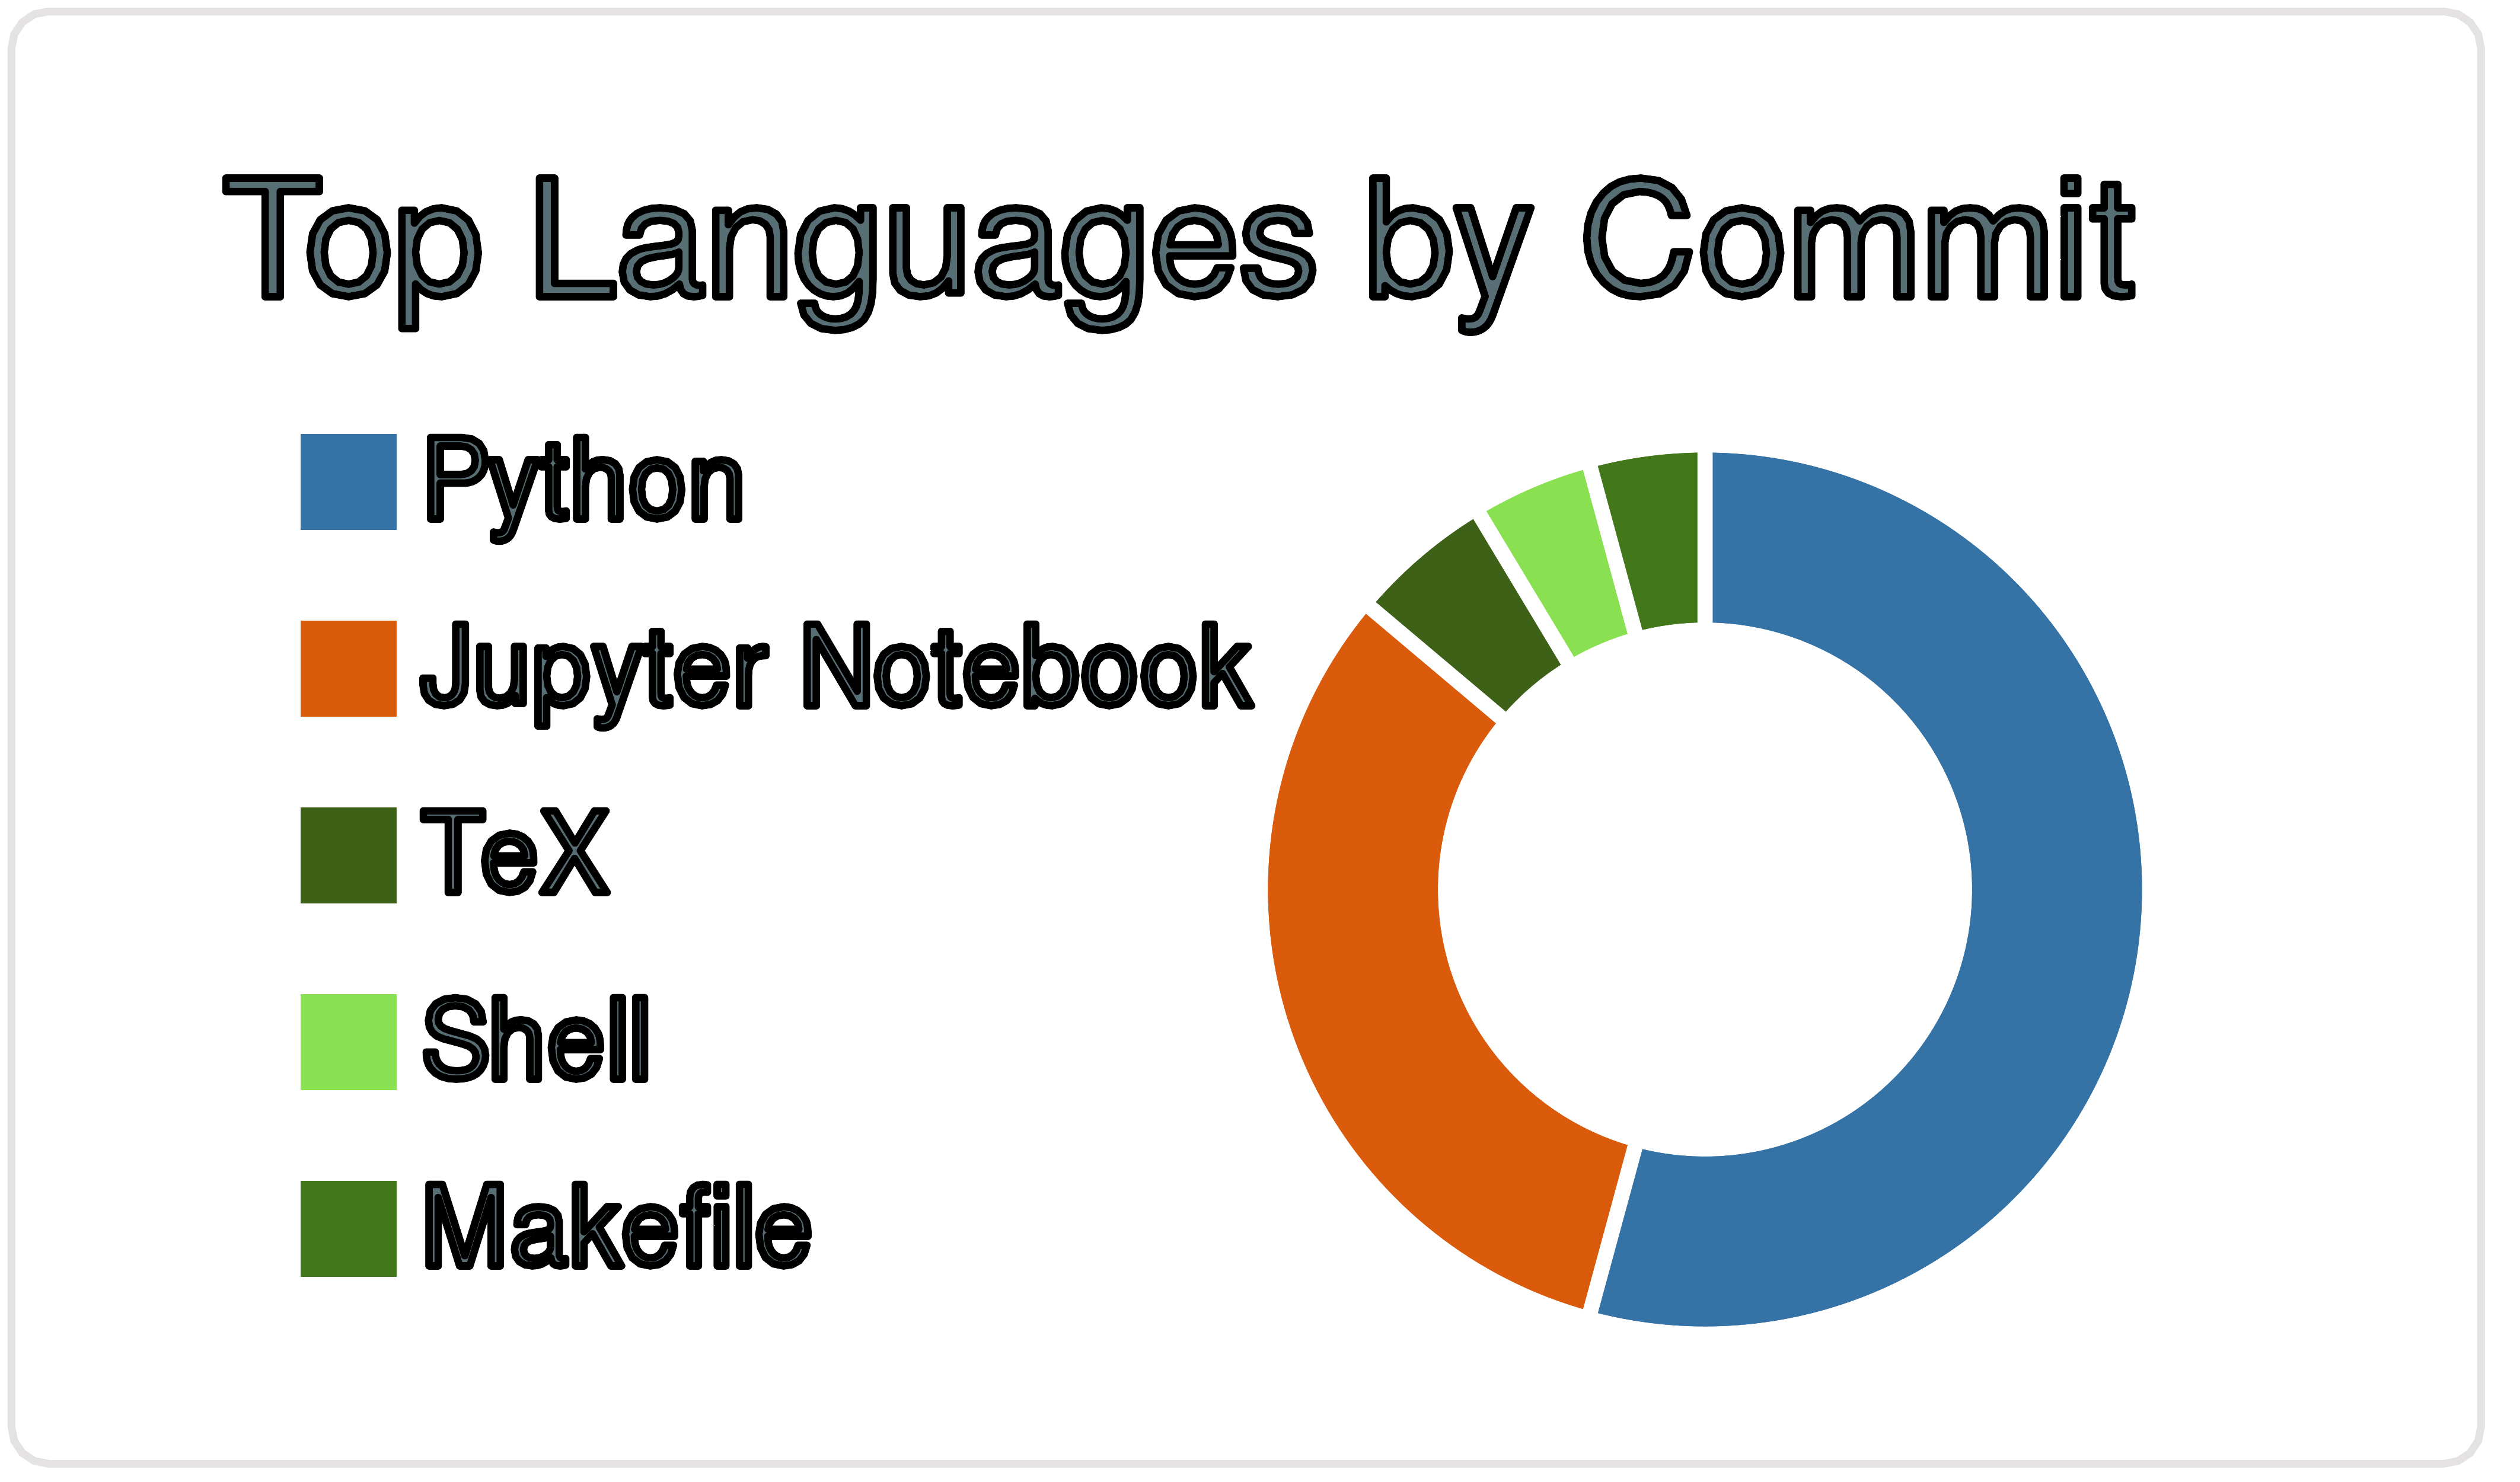
\includegraphics[width=0.50\linewidth]{2-most-commit-language.png}
\end{textblock*}
\note{My Twitter and Github accounts are \href{https://twitter.com/tkoyama010}{@tkoyama010}.}
\note{Please follow me if you like this presentation.}
\end{frame}

\end{document}


